\chapter{Cloudbreak}\label{chap_cloudbreak_impl}

Cloudbreak is our implementation, in the framework described above, of a detection algorithm for genomic deletions (40bp-25,000bp) and small insertions based on examining the insert sizes of paired end mappings. Cloudbreak is a native Java Hadoop application. We deployed Cloudbreak on a 56-node cluster running the Cloudera CDH3 Hadoop distribution, version 0.20.2-cdh3u4. We use snappy compression for MapReduce data, and Hadoop's distributed cache mechanism to share the executable files and indices needed for mapping tasks to the nodes in the cluster. An illustration of the Cloudbreak algorithm working on a simple example is shown in Figure \ref{cloudbreak_example}.

\begin{figure}
\centering
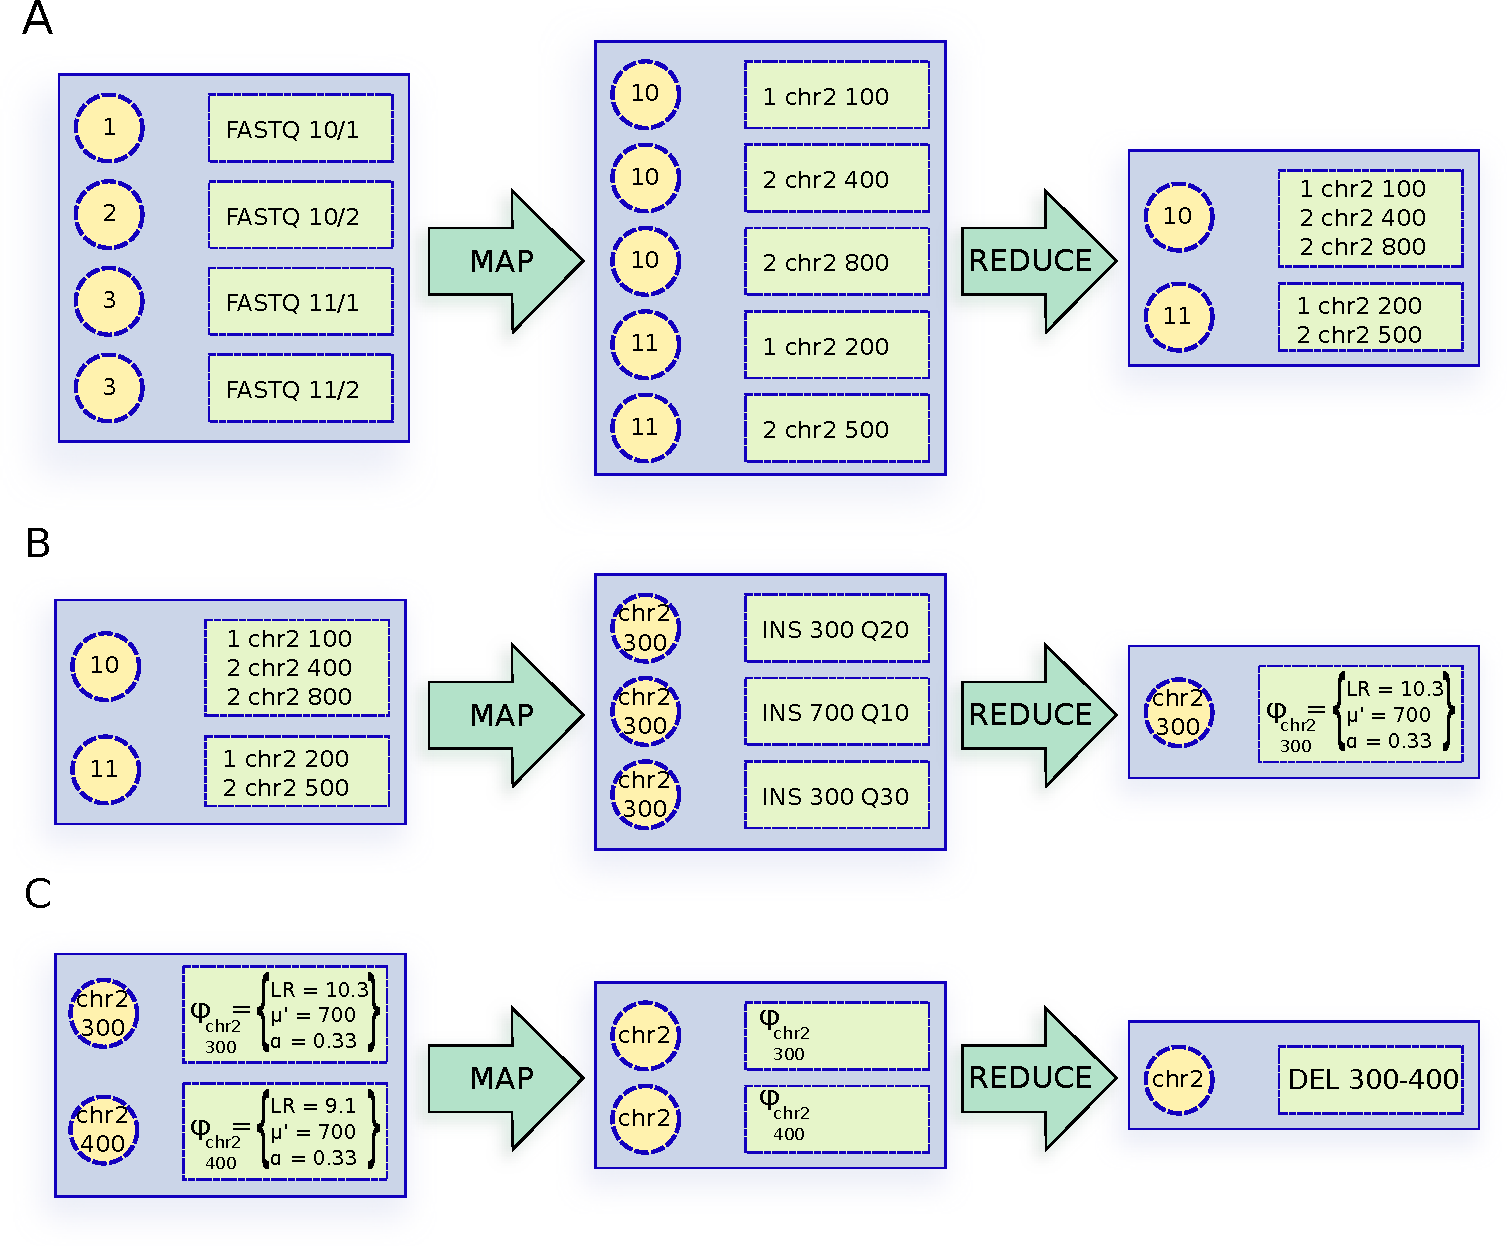
\includegraphics[width=.9\textwidth]{/users/cwhelan/Documents/svpipeline/figures/cloudbreak_mapred_diagram.pdf}
\caption{An Example of the Cloudbreak MapReduce Algorithm. A) In the first MapReduce job, mappers scan input reads in FASTQ format and execute an alignment program in either paired-end or single-ended mode to generate read mappings. Reducers gather all alignments for both reads in each pair. B) In the second MapReduce job, mappers first emit information about each read pair (in this case the insert size and quality) under keys indicating the genomic location spanned by that pair. Only one genomic location is diagrammed here for simplicity. Reducers then compute features for each location on the genome by fitting a GMM to the distribution of spanning insert sizes. C) Mappers group all emitted features by their chromosome, and reducers find contiguous blocks of features that indicate the presence of a variant.}
\label{cloudbreak_example}
\end{figure}


\section{Implementation of the MapReduce SV Framework}

In particular, we implement the three user-defined functions specified above as follows:

\begin{description}
\item[\sc{Loci}] Because we are detecting deletions and short insertions, we map ReadPairInfos from each possible alignment to the genomic locations overlapped by the implied internal insert between the reads. For efficiency, we define a maximum detectable deletion size of 25,000bp, and therefore alignment pairs in which the ends are more than 25kb apart, or in the incorrect orientation, map to no genomic locations. In addition, if there are multiple possible mappings for each read in the input set, we optimize this step by assuming that if there exists a concordant mapping for a read pair, defined as a mapping pair in which the two alignments are in the proper orientation and with an insert size within three standard deviations of the expected library insert size, it is likely to be correct and therefore we do not consider any discordant alignments of the pair.

\item[$\Phi$] To compute features for each genomic location, we follow Lee et al. \cite{Lee:2009da}, who observed that if all mappings are correct, the insert sizes implied by mappings which span a given genomic location should follow a Gaussian mixture model (GMM) whose parameters depend on whether a deletion or insertion is present at that locus (Figure A1). Briefly: if there is no indel, the insert sizes implied by spanning alignment pairs should follow the distribution of actual fragment sizes in the sample, which is typically modeled as normally distributed with mean $\mu$ and standard deviation $\sigma$. If there is a homozygous deletion or insertion of length $l$ at the location, $\mu$ should be shifted to $\mu + l$, while $\sigma$ will remain constant. Finally, in the case of a heterozygous event, the distribution of insert sizes will follow a mixture of two normal distributions, one with mean $\mu$, and the other with mean $\mu + l$, both with an unchanged standard deviation of $\sigma$, and mixing parameter $\alpha$ that describes the relative weights of the two components. The features generated for each location $l$ include the log-likelihood ratio of the filtered observed data points under the fit GMM to their likelihood under the distribution $N(\mu,\sigma)$, the final value of the mixing parameter $\alpha$, and $\mu'$, the estimated mean of the second GMM component. 

At each genome location, we fit the parameters of the GMM using the Expectation-Maximization algorithm. Let $Y = y_{1,2, \ldots m}$ be the observed insert sizes at each location after filtering, and say the library has mean fragment size $\mu$ with standard deviation $\sigma$. Because the mean and standard deviation of the fragment sizes are selected by the experimenter and therefore known \emph{a priori} (or at least easily estimated based on a sample of alignments), we only need to estimate the mean of the second component at each locus, and the mixing parameter $\alpha$. Therefore, we initialize the two components to have means $\mu$ and $\bar{Y}$, set the standard deviation of both components to $\sigma$, and set $\alpha = .5$. In the E step, we compute for each $y_i$ and GMM component $j$ the value $\gamma_{i,j}$, which is the normalized likelihood that $y_i$ was drawn from component $j$. We also compute $n_j = \sum_i{\gamma_{i,j}}$, the relative contributions of the data points to each of the two distributions. In the M step, we update $\alpha$ to be $n_2 - \left|Y\right|$, and set the mean of the second component to be $\frac{\sum_m{\gamma_{m,2}y_m}}{n_2}$. We treat the variance as fixed and do not update it, since under our assumptions the standard deviation of each component should always be $\sigma$. We repeat the E and M steps until convergence, or until a maximum number of steps has been taken.

Prior to fitting the GMM at each location, we attempt to filter our incorrect mappings for that location using an outlier-detection based clustering scheme and an adaptive mapping quality cutoff.

\item[\sc{PostProcess}] The third MapReduce job is responsible for making SV calls based on the feature defined above. We convert our features along each chromosome to insertion and deletion calls by first extracting contiguous genomic loci where the log-likelihood ratio of the two models is greater than a given threshold. To eliminate noise we apply a median filter with window size 5. We end regions when $\mu'$ changes by more than 60bp ($2\sigma$), and discard regions where the average value of $\mu'$ is less than $\mu$ or where the length of the region differs from $\mu'$ by more than $\mu$.
\end{description}


\begin{figure}
\centering
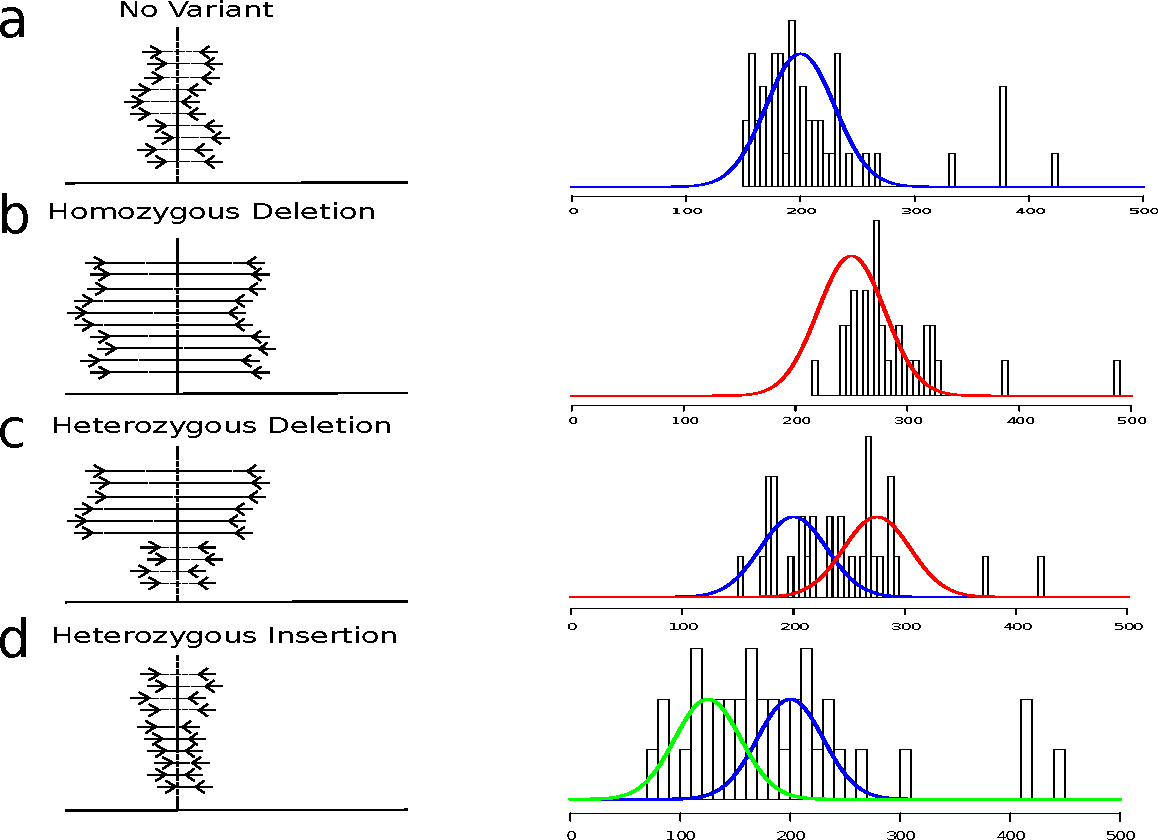
\includegraphics[width=.9\textwidth]{figures/insert_size_mixtures.pdf}
\caption{Illustration of insert size mixtures at individual genomic locations. A) there is no variant present at the location indicated by the vertical line (left), so the mix of insert sizes (right) follows the expected distribution of the library centered at 200bp, with a small amount of noise coming from low-quality mappings. B) a homozygous deletion of 50bp at the location has shifted the distribution of observed insert sizes. C) A heterozygous deletion at the location causes a mixture of normal and long insert sizes to be detected. D) A heterozygous small insertion shifts a portion of the mixture to have lower insert sizes.}
\label{insert_size_mixes}
\end{figure}


\section{Incorrect and ambiguous mappings}

To handle incorrect and ambiguous mappings, we assume that in general they will not form normally distributed clusters in the same way that correct mappings will, and therefore use an outlier detection technique to filter the observed insert sizes for each location. We sort the observed insert sizes and define as an outlier an observation whose $k$th nearest neighbor is more than $n\sigma$ distant, where $k = 3$ and $n = 5$. In addition, we rank all observations by the estimated probability that the mapping is correct and use an \emph{adaptive quality cutoff} to filter observations: we discard all observations where the estimated probability the mapping is correct is less than the score of the maximum quality observation minus a constant $c$. This allows the use of more uncertain mappings in repetitive regions of the genome while restricting the use of low-quality mappings in unique regions. Defining $\textsc{Mismatches}(a)$ to be the number of mismatches between a read and the reference genome in the alignment $a$, we approximate the probability $p^{k}_c$ of each end alignment being correct by:

\[ p^{k}_c(a^{k}_{m,i}) = \frac{\exp({-\textsc{Mismatches}(a^{k}_{m,i})/2)}}{\sum_j{\exp(-\textsc{Mismatches}(a^{k}_{m,j})/2)}} \]

And then multiply $p_c(a^{1}_{m,i})$ and $p_c(a^{2}_{m,i})$ to approximate the likelihood that the pair is mapped correctly.

\section{Genotyping}

In theory, it should be possible to use the parameters of the fit GMM to infer the genotype of each predicted variant. Assuming that our pipeline is capturing all relevant read mappings near the locus of the variant, the genotype should be indicated by the estimated parameter $\alpha$, the mixing parameter that controls the weight of the two components in the GMM. We set a simple cutoff of .35 on the average value of $\alpha$ for each prediction to call the predicted variant homozygous or heterozygous, and use the same cutoff for deletion and insertion predictions.
